\section{Лекция 9. Дополнительное условие выпуклости и дифференцируемости, ККТ}

\subsection{Нормальный конус для регулярной тройки}
\textbf{Лемма 3.11}\\
Если $(X_{0},(g_{(i)})_{i\in[m]},(h_{(i)})_{i\in[p]})$ регулярная, тогда:
\begin{center}
    $N_{x*}(X) = N_{x*}(X_{0}) + \sum_{i\in[m]}{N_{x*}(G_{i})} + \sum_{i\in[p]}{N_{x*}(H_{i})}$.\\
\end{center}
$(X_{0},(g_{(i)})_{i\in[m]},(h_{(i)})_{i\in[p]})$ регулярная если:
\begin{enumerate}
    \item Множество $X_{0}$ -- полиэдр и функции $g_{1},\ldots,g_{m}$ аффинные\\ или
    \item Множество $X\bigcap int(X_{0})$ не пусто и функции $g_{1},\ldots,g_{m}$ аффинные\\ или
    \item Существует точка $x^{(s)} \in X$ $(x^{(s)} \in int(X_{0}), если p \neq 0)$ такая, что $g_{i}(x^{(s)}) < 0$ для всех $i\in[m]$ (условие Слейтера)\\
\end{enumerate}


\subsection{Дополнительное условие выпуклости и дифференцируемости}
{\bf Теорема 1.16}

Если $ g: \mathbb{R}^n\rightarrow \mathbb{R}$  дифференцируемая, выпуклая и существует точка $x^{(s)}\in \mathbb{R}^n$ такая, что $g(x^{(s)})<0$, то для всех $x^{*}\in \mathbb{R}^n$, для которых $g(x^{*})\leq 0$:


$N_{x^{*}}(g^{-1}(\mathbb{R_-}))=$
$$\displaystyle
\begin{cases} cone\{grad_{x^*} g\},  g(x^*)=0 \\ \{\mathbb{O}_n\},  g(x^*)<0 \end{cases}$$


{\bf Доказательство}
\begin{enumerate}
    \item Сначала определим множество $G:=g^{-1}(\mathbb{R_-})=\{x\in \mathbb{R^n}:g(x)\leq 0\}$.\\

    \begin{itemize}
        \item Предположим, что точка $x^{(s)}\in \mathbb{R^{n}}$, такая что $g(x^{(s)}<0)$, существует.

     \item Если $g(x^*)<0$, тогда $x^{(s)}\in int(G)$ (Так как, если непрерывная функция меньше нуля в конкретной точке, то она меньше нуля и в некоторой окрестности этой точки.)\\
        И, также, $N_{x^{*}}(G)=\{\mathbb{O}\}$
     Пусть теперь $g(x^*)=0$. Нужно показать, что $N_{x^{*}}(G)=cone\{grad_{x^*} g\}$\\
    \end{itemize}
    \item "$\supseteq$"
     \begin{itemize}

     \item Покажем, что $N_{x^{*}}(G)\supseteq cone\{grad_{x^*} g\}$ т.е. надо показать, что градиент содержится в нормальном конусе, так как $cone\{grad_{x^*} g\}$ содержит градиент\\
        Будем доказывать от противного. Положим, что
        $$cone\{grad_{x^*} g\}\notin N_{x^{*}}(G)=(cone (G-\{x^*\}))^\circ $$
        \item Соответственно, существует $x\in G$ такой, что $<grad_{x^* g},x-x^*>>0$
        (Так как в поляре лежат все векторы, которые более чем ортогональны с исходным. А само это утверждение вытекает из предположения, что градиент не лежит в поляре.)\\
        Значит, существуют точки на сколь угодно большом расстоянии от $x^*$ такие, что их можно выразить следующим образом $y(t)=x^*+t(x-x^*)$ с $g(y(t))>g(x^*)$ $(t\geq 0 )$

     \item Далее выберем такое $t$, что $0\leq t\leq 1 \Rightarrow g(y(t))>g(x^*)=0$\\
        С другой стороны $y(t)\in conv\{x^*,x\}\supseteq G$. Но на множестве $G g(x)\leq 0$. Получили противоречие.
        \end{itemize}
        \item "$\subseteq$"
        \begin{itemize}
       \item Достаточно показать, что для всех $y\in \mathbb{R^n}$ таких, что $<grad_{x^*} g,y>\leq 0$: $y\in cl(K_{x^*}(G))$\\
            (Так как $(cone\{grad_{x^*} g\})^\circ \subseteq cl(K_{x^*}(G))$)
        Следовательно $N_{x^*}(G)=(K_{x^*}(G))^\circ=(cl(K_{x^*}(G)))^\circ \subseteq ((cone(grad_{x^*} (g))^\circ)^\circ = cone{grad_{x^*}(g)}$

             \begin{center} 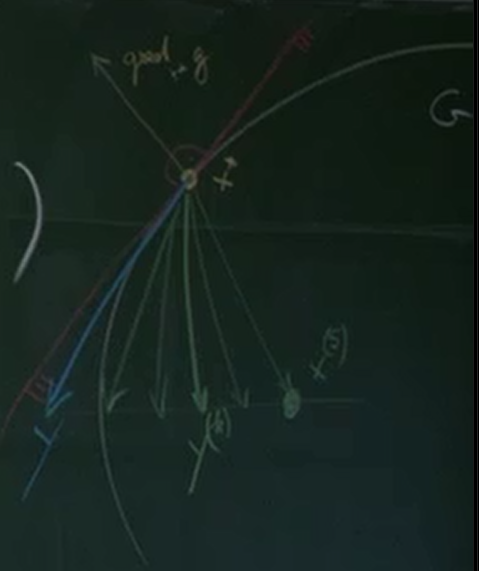
\includegraphics[scale=0.5]{png2}
         \end{center}



         \item ПОЯСНЕНИЯ. Любой вектор, который более чем ортогонален градиенту, должен лежать в допустимом направлении или, по крайней мере, в замыкании допустимых направлений, исходящих из $x^*$. Если $<grad_{x^*},y>=0$ - это недопустимое направление, но $y$ лежит в топологическом замыкании допустимых направлений. Мы строим последовательность векторов, которые гарантированно лежат в радиальном конусе и сходятся к $y$. И тут нам нужна точка $x^{(s)}$ из условий теоремы, которая точно лежит в $G$.
         \item Пусть $y\in \mathbb{R}^n$ такой, что $<grad_{x^*},y>\leq 0$
         \item Определим последовательность $y^{(k)}:=\frac{1}{k}(x^{(s)}-x^*)+\frac{k-1}{k}y$. Заметим, что все $y^{(k)}$ лежат в радиальном конусе.
         \item Так как $\displaystyle \lim_{k \to \infty} y^k = y$ достаточно показать, что для всех $k y^{(k)}\in K_{x^*}(G)$.
         \item $<grad_{x^*} g, y^{(k)}>=\frac{1}{k}<grad_{x^*}g,x^{(s)-x^*}>+\frac{k-1}{k}<grad_{x^*}g,y>$
             \\ Первое слагаемое строго меньше нуля( $g(x^*)=0, g(x^{(s)}<0), g - $ выпуклая), а второе меньше либо равно.
         \item Получаем $<grad_{x^*}g,y^{(k)}><0$, т.е. функция $g$ убывает в направлении $y^{(k)}$, т.е. на любом расстоянии от $x^*$ много меньших значений функции $g$.\\
         Следовательно, существует $t>0$, c $g(x^*+t y^{(k)})<0$ и $y^{(k)}\in cone\{x-x^*\}\subseteq cone\{cone(G-\{x^*\})\}=K_{x^*}(G)$.
         \end{itemize}
         \begin{flushright} $\square$
         \end{flushright}
\end{enumerate}

\subsection{Условия Каруша - Кунна - Такера (дифференцируемость, выпуклость)}
{\bf Теорема 3.13}\\ Точка $x^{*} \in X$ является оптимальным решением задачи \begin{equation*} min\left\lbrace f(x) | x\in X \right\rbrace \end{equation*} когда $\exists$ множители $\lambda_1,..,\lambda_m \in \mathbb{R_{+}}$ и $\mu_1,..,\mu_p \in \mathbb{R}$ такое, что \begin{equation*} \tag{1} grad_{x^{*}}f + \displaystyle\sum_{i=1}^{m} \lambda_i grad_{x^{*}}g_i + \displaystyle\sum_{i=1}^{p} \mu_i grad_{x^{*}}h_i \in - N_{x^{*}}\left(x_0\right) \end{equation*} и \begin{equation*} \tag{2} \lambda_i=0 \text{ для всех } i \in \left[m\right] \text{, что } g_i\left(x^{*}\right)<0 \end{equation*}
 \subsection{Условия Каруша - Кунна - Такера для задачи линейной оптимизации (1 вариант)}
 {\bf Теорема 3.14 (Условия дополняющей нежесткости 1)}\\
 Пусть $A\in \mathbb{R}^{m*n}, b\in\mathbb{R}^m$ и $c\in\mathbb{R}^n$. Точка $x^*\in \mathbb{R}^n_+$ с $Ax^*=b$ является оптимальным решением задачи
 $$\min{\{<c,x>|Ax=b,x\in\mathbb{R}^n_+\}},$$
когда существует $\mu\in\mathbb{R}^m$ с $\mu^T<=c^T$ и
$$\mu^T A_{*,j}=c_j, j\in[n], x^{*}_{+}>0.$$

Теорема 3.14 следует из теоремы 3.13 с $f(x)=<c,x>,x_0; x_0\in \mathbb{n}_+, m=0, h_i(x)=<A_{i,*}x>-b_i (i\in[p])$ - начальные условия. $\Rightarrow$ регулярно (тип 1), $X_0$ - полиэдр.
Проверка выполнения условий теоремы 3.13:
(2) ${\o}$, т.к. m=0
(1) $\displaystyle c+\sum_{i=1}^{p}\mu A_{i,*}\in\{-x: x\in \mathbb{R}^n_-, <x,x^*>=0\}$(Лемма 3.8) $\Leftrightarrow c-\overline{\mu}^T A\in \{x\in\mathbb{R}^{n}_{+}, <x,x_*>=0\} \Leftrightarrow c-\overline{\mu}^T A\geq$ и с $c_j-\overline{\mu}^T A_{*,j}=0 \forall j\in[n], x^{*}{j}>0$.

\subsection{ККТ для задачи линейной оптимизации (2 вариант)}

{\bf Теорема 3.15}\\
Пусть $A\in\mathbb{R}^{m*n},b\in\mathbb{R}^n, c\in\mathbb{R}^n$, точка $x^*\in\mathbb{R}^n, Ax^*\leq b$ является решением задачи:
$$\max{\{<c,x>|Ax\leq b, x\in\mathbb{R}^n\}},$$
тогда $\exists$ вектор $\lambda\in\mathbb{R}^{m}_{+}, \lambda^T A=c^T$ и
$$\lambda_i=0б i\in[m], <A_{i,*},x^*><b_i$$ 